\documentclass{beamer}

\usepackage{verbatim}
\usepackage{fancyvrb}
\usepackage{amsmath}
\usepackage{mathtools}
\usepackage{booktabs}
\usepackage{amssymb}
\usepackage{graphicx}
\usepackage{calc}
\usepackage{color}
\usepackage{multicol}
\usepackage{wrapfig}
\usepackage{natbib}
\usepackage[ruled,vlined]{algorithm2e}
\usepackage{animate}
\usepackage{mathtools}
\usepackage{listings}

\usepackage{cmbright}
\fontencoding{OT1}\fontfamily{cmbr}\selectfont %to load ot1cmbr.fd
\DeclareFontShape{OT1}{cmbr}{bx}{n}{% change bx definition
<->cmbrbx10%
}{}
\normalfont % back to normalfont

% two col: two columns
\newenvironment{twocol}[4]{
\begin{columns}[c]
\column{#1\textwidth}
#3
\column{#2\textwidth}
#4
\end{columns}
}

\makeatletter
\setbeamertemplate{theorem begin}
{%
\begin{\inserttheoremblockenv}
  {}{\usebeamerfont*{block title}\usebeamercolor[fg]{block title}%
  \inserttheoremname
  %\inserttheoremnumber
  \ifx \inserttheoremaddition \empty \else\ (\inserttheoremaddition)\fi
  \inserttheorempunctuation}
  \normalfont
  }
  \setbeamertemplate{theorem end}{\end{\inserttheoremblockenv}}
\makeatother

\newcommand{\E}{\mathrm{E}}
\newcommand{\Var}{\mathrm{Var}}
\newcommand{\Cov}{\mathrm{Cov}}
\newcommand{\sd}{\mathrm{sd}}
\newcommand{\s}{\mathrm{s}}
\newcommand{\Corr}{\mathrm{Corr}}
\newcommand{\rank}{\mathrm{rank}}
\newcommand{\trace}{\mathrm{trace}}
\newcommand{\nullspace}{\mathrm{null}}
\newcommand{\myspan}{\mathrm{span}}
\DeclareMathOperator*{\argmax}{arg\,max}
\DeclareMathOperator*{\argmin}{arg\,min}
\DeclareMathOperator*{\softmax}{softmax}

\definecolor{darkgreen}{rgb}{0,0.5,0}

\newtheorem{proposition}[theorem]{Proposition}
\newtheorem{exe}{Exercise}
\newtheorem{notation}{Notation}
\newtheorem{remark}{Remark}

\definecolor{darkgreen}{rgb}{0,0.5,0}
\title{Multiple Regression I}
\author{Zhenisbek Assylbekov}
\institute{Department of Mathematics}
\date{Regression Analysis}

\AtBeginSection[]
{
  \begin{frame}<beamer>
    \tableofcontents[currentsection]
  \end{frame}
}

\begin{document}

\begin{frame}
  \titlepage
\end{frame}

\begin{frame}{Multiple regression models}
We now add more predictors, linearly, to the model. \pause For example let's add one more to the simple linear regression model:
$$
Y_i=\beta_0+\beta_1 x_{i1}+\beta_2 x_{i2}+\epsilon_i,\qquad \epsilon_i\,\,{\stackrel{\text{iid}}{\sim}}\,\,\mathcal{N}(0,\sigma^2)
$$
\pause For \textit{any} $Y$ in this population with predictors $(x_1,x_2)$ we have
$$
\E[Y]=\beta_0+\beta_1 x_1 + \beta_2 x_2
$$
\pause This is an equation of a plane in $\mathbb{R}^3$.

\pause \begin{figure}
    \centering
    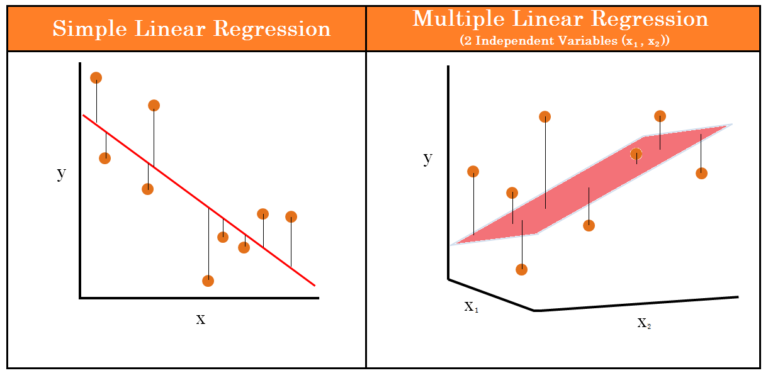
\includegraphics[height=.4\textheight]{plots/reg_plane.png}
\end{figure}
\end{frame}

\begin{frame}{Multiple regression models}
Generally, for $k=p-1$ predictors $x_1,\ldots,x_k$ our model is
$$
Y_i=\beta_0+\beta_1 x_{i1}+\beta_2 x_{i2} + \cdots + \beta_k x_{ik} + \epsilon_i,
$$
where
\begin{itemize}
\item\pause $\beta_0$ is \pause mean response when all predictors equal zero (if this makes sense).
\item\pause $\beta_j$ is \pause the change in mean response when $x_j$ is increased by one unit \textit{but the remaining predictors are held  constant}.
\item\pause We will assume normal errors:
$$
\epsilon_1, \ldots, \epsilon_n\stackrel{\text{ iid}}{\sim}\mathcal{N}(0, \sigma^2).
$$
\end{itemize}
\end{frame}

\begin{frame}{Example: Dwayne Portrait Studio data}
Dwaine Studios, Inc., operates portrait studios in 21 cities of medium size. \pause These studios
specialize in portraits of children. \pause The company is considering an expansion into other
cities of medium size and wishes to investigate whether sales ($Y$) in a community can be
predicted from the number of persons aged 16 or younger in the community ($x_1$) and the
per capita disposable personal income in the community ($x_2$).\\~\\

Assume the linear model is appropriate. One way to check marginal relationships is through a scatterplot matrix. %However, these are not infallible.

%For these data, is $\beta_0$ interpretable?

%$\beta_2$ is the change in the mean response for a thousand-dollar increase in disposable income, holding ``number of people under 16 years old'' constant.
\end{frame}


\begin{frame}{Scatterplot matrix}
{\url{https://github.com/zh3nis/MATH440/blob/main/chp06/scatter_matrix.R}}

\centering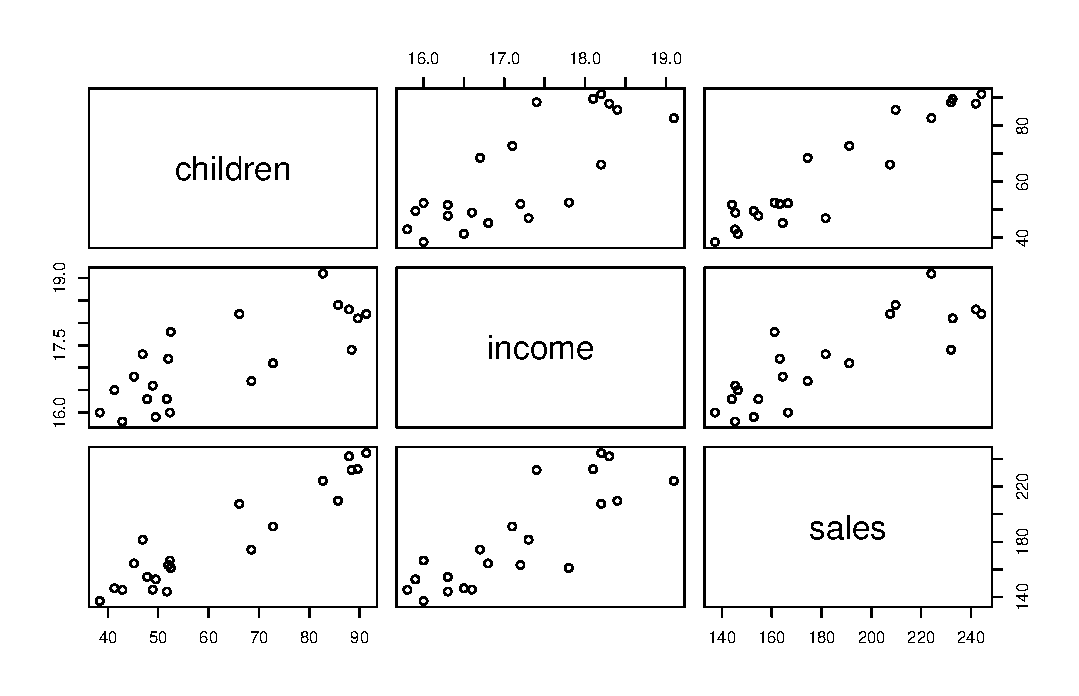
\includegraphics[width=\textwidth]{plots/scatter_matrix.pdf}
\end{frame}

\begin{frame}{The general linear model encompasses\ldots}

\structure{Qualitative predictors}

We can use dummy variables to represent qualitative predictors.

\pause \begin{example}
Binary predictor
\begin{itemize}
\item\pause $Y = $ length of hospital stay
\item\pause $x_1= $ gender of patient ($x_1=0$ male, $x_1=1$ female)
\item\pause $x_2= $ severity of a disease on 100 point scale
\pause $$
\E[Y]=\begin{cases}
\beta_0+\beta_1\cdot0+\beta_2 x_2\quad &\text{males}\\
\beta_0+\beta_1\cdot1 + \beta_2 x_2\quad &\text{females}.
\end{cases}
$$
\pause Response functions are two parallel lines, shifted by $\beta_1$ units.
\end{itemize}
\end{example}
\end{frame}


\begin{frame}{The general linear model encompasses\ldots}

\structure{Polynomial regression}

\pause Often appropriate for curvilinear relationship between response and predictor

\pause \begin{example}
$$
Y=\beta_0+\beta_1 x_1 + \beta_2 x_1^2 + \epsilon.
$$
\pause Letting $x_2=x_1^2$ this is in the form of the general linear model.
\end{example}
\vspace{20pt}

\pause \structure{Transformed response}

\pause \begin{example}
$$
\log Y=\beta_0+\beta_1 x_1 + \beta_2 x_2 + \beta_3 x_3 + \epsilon.
$$
\pause Let $Y^\ast=\log Y$ and get general linear model.
\end{example}
\end{frame}

\begin{frame}{The general linear model encompasses\ldots}
\structure{Interaction effects}
\pause \begin{example}
$$
Y=\beta_0+\beta_1 x_1 + \beta_2 x_2 + \beta_3 x_1 x_2 + \epsilon.
$$
\pause Let $x_3=x_1 x_2$ and get general linear model.
\end{example}
\hrulefill

\pause All of these models are \textit{linear in the coefficients}, the $\beta_j$ terms. \pause An example of a model that is \textit{not} in general linear model form is exponential growth:
$$
Y=\beta_0\exp(\beta_1 x)+\epsilon.
$$

\end{frame}


\begin{frame}
\frametitle{Another example with a binary predictor -- weights of books}

\twocol{0.6}{0.4}{
{\small
\begin{center}
\begin{tabular}{rrrc}
  \hline
 & weight (g) & volume (cm$^\text{3}$) & cover \\ 
  \hline
1 & 800 & 885 & hc \\ 
  2 & 950 & 1016 & hc \\ 
  3 & 1050 & 1125 & hc \\ 
  4 & 350 & 239 & hc \\ 
  5 & 750 & 701 & hc \\ 
  6 & 600 & 641 & hc \\ 
  7 & 1075 & 1228 & hc \\ 
  8 & 250 & 412 & pb \\ 
  9 & 700 & 953 & pb \\ 
  10 & 650 & 929 & pb \\ 
  11 & 975 & 1492 & pb \\ 
  12 & 350 & 419 & pb \\ 
  13 & 950 & 1010 & pb \\ 
  14 & 425 & 595 & pb \\ 
  15 & 725 & 1034 & pb \\ 
   \hline
\end{tabular}
\end{center}
}}
{
\begin{center}
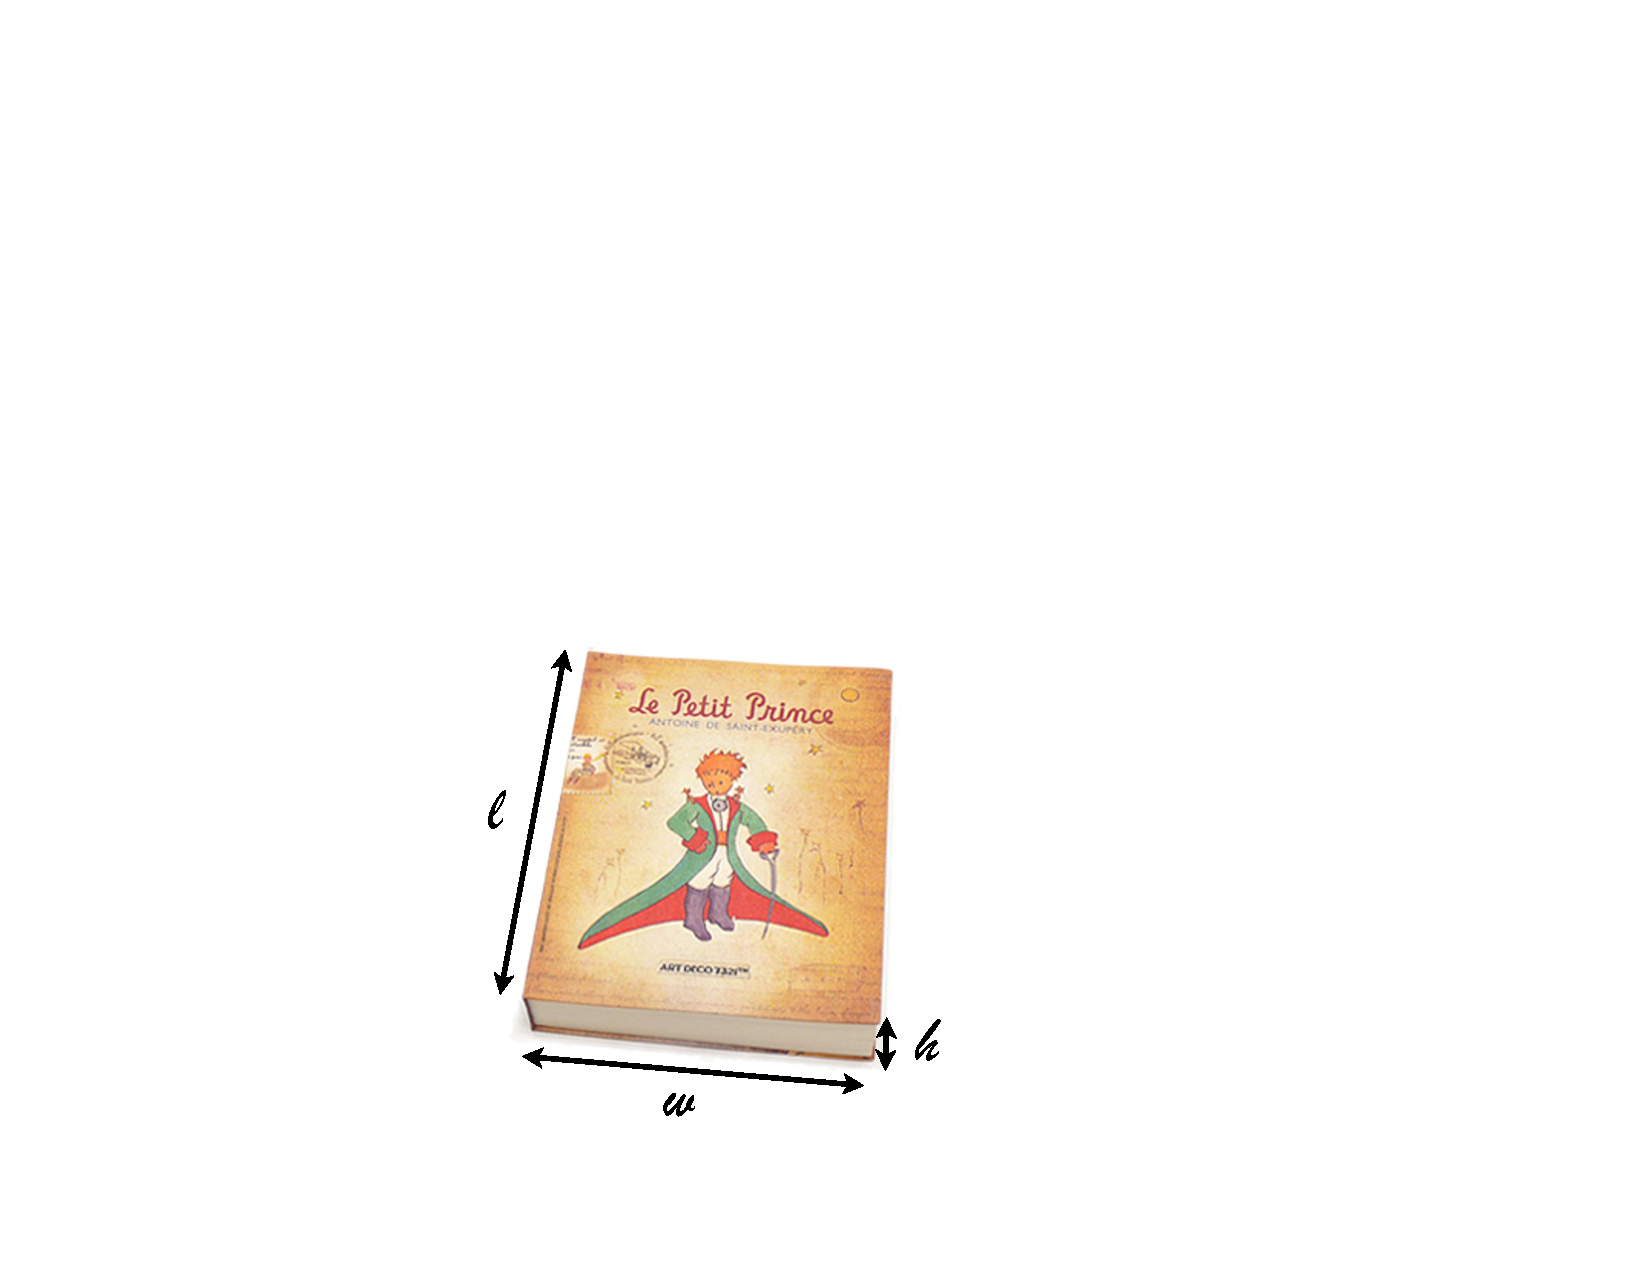
\includegraphics[width=0.7\textwidth]{plots/book}
\end{center}
}

{\footnotesize(From: Maindonald, J.H. and Braun, W.J. (2nd ed., 2007) ``Data Analysis and Graphics Using R")}

\end{frame}

%%%%%%%%%%%%%%%%%%%%%%%%%%%%%%%%%%%

\begin{frame}
\frametitle{Weights of books (cont.)}

\begin{columns}
\begin{column}{0.45\textwidth}
{\small The scatterplot shows the relationship between weights and volumes of books as well as the regression output. Which of the below is correct?}
\end{column}
\begin{column}{0.45\textwidth}
\begin{center}
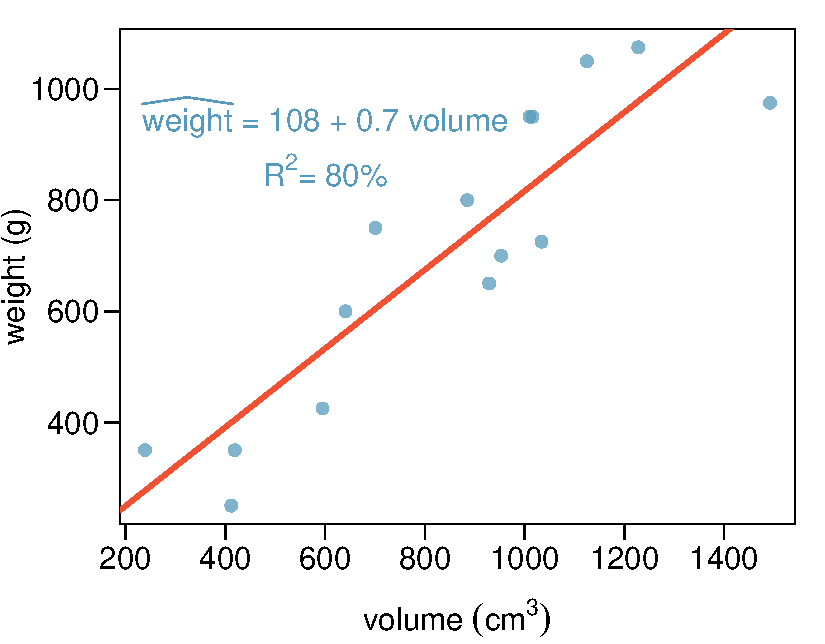
\includegraphics[width=\textwidth]{plots/weight_volume}
\end{center}
\end{column}
\end{columns}


\begin{enumerate}[(a)]
\item \pause Weights of 80\% of the books can be predicted accurately using this model.
\item \pause Books that are 10 cm$^\text{3}$ over average are expected to weigh 7 g over average.
\item \pause The correlation between weight and volume is $R = 0.80^2 = 0.64$.
\item \pause The model underestimates the weight of the book with the highest volume.
\end{enumerate}

\end{frame}

%%%%%%%%%%%%%%%%%%%%%%%%%%%%%%%%%%%

\begin{frame}[fragile]
\frametitle{Modeling weights of books using only volume}

\begin{verbatim}
Coefficients:
             Estimate Std. Error t value Pr(>|t|)    
(Intercept) 107.67931   88.37758   1.218    0.245    
volume        0.70864    0.09746   7.271 6.26e-06


Residual standard error: 123.9 on 13 degrees of freedom
Multiple R-squared: 0.8026,	Adjusted R-squared: 0.7875 
F-statistic: 52.87 on 1 and 13 DF,  p-value: 6.262e-06 
\end{verbatim}

\end{frame}

%%%%%%%%%%%%%%%%%%%%%%%%%%%%%%%%%%%

\begin{frame}
\frametitle{Weights of hardcover and paperback books}

Can you identify a trend in the relationship between volume and weight of hardcover and paperback books?

\only<2>{\small Paperbacks generally weigh less than hardcover books after controlling for the bookÕs volume.}

\begin{center}
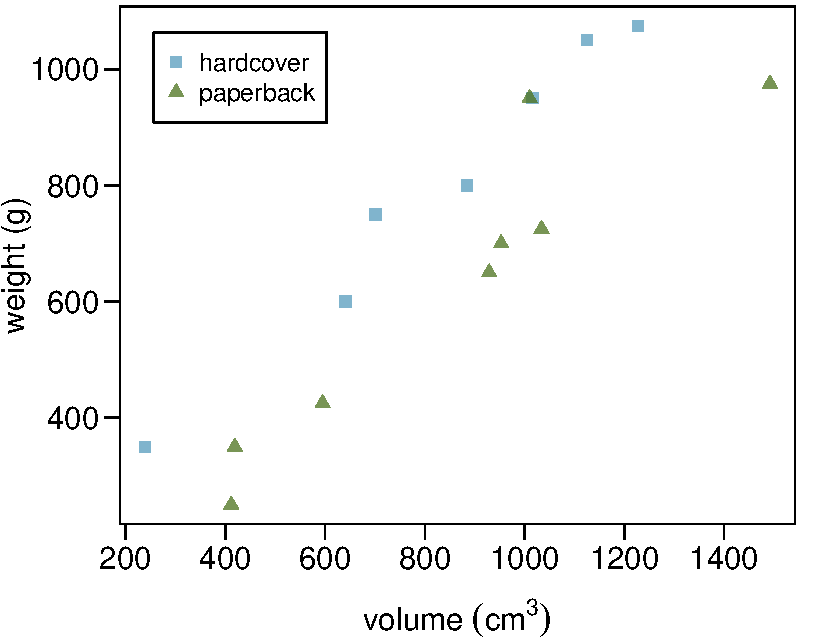
\includegraphics[width=0.6\textwidth]{plots/weight_volume_cover}
\end{center}

\end{frame}

%%%%%%%%%%%%%%%%%%%%%%%%%%%%%%%%%%%

\begin{frame}[fragile]
\frametitle{Modeling weights of books using volume \underline{and} cover type}

\begin{verbatim}
Coefficients:
              Estimate Std. Error t value Pr(>|t|)    
(Intercept)  197.96284   59.19274   3.344 0.005841 ** 
volume         0.71795    0.06153  11.669  6.6e-08 ***
cover:pb    -184.04727   40.49420  -4.545 0.000672 ***


Residual standard error: 78.2 on 12 degrees of freedom
Multiple R-squared: 0.9275,	Adjusted R-squared: 0.9154 
F-statistic: 76.73 on 2 and 12 DF,  p-value: 1.455e-07 
\end{verbatim}

\end{frame}

%%%%%%%%%%%%%%%%%%%%%%%%%%%%%%%%%%%

\begin{frame}
\frametitle{Determining the reference level}

Based on the regression output below, which level of \tt{cover} is the reference level? Note that \tt{pb}: paperback.

{\small
\begin{center}
\begin{tabular}{rrrrr}
  \hline
 & Estimate & Std. Error & t value & Pr($>$$|$t$|$) \\ 
  \hline
(Intercept) & 197.9628 & 59.1927 & 3.34 & 0.0058 \\ 
  volume & 0.7180 & 0.0615 & 11.67 & 0.0000 \\ 
  cover:pb & -184.0473 & 40.4942 & -4.55 & 0.0007 \\ 
   \hline
\end{tabular}
\end{center}
}

\begin{enumerate}[(a)]
\item paperback
\item hardcover
\end{enumerate}

\end{frame}

%%%%%%%%%%%%%%%%%%%%%%%%%%%%%%%%%%%

\begin{frame}
\frametitle{Linear model}

{\small
\begin{center}
\begin{tabular}{rrrrr}
  \hline
 & Estimate & Std. Error & t value & Pr($>$$|$t$|$) \\ 
  \hline
(Intercept) & 197.96 & 59.19 & 3.34 & 0.01 \\ 
  volume & 0.72 & 0.06 & 11.67 & 0.00 \\ 
  cover:pb & -184.05 & 40.49 & -4.55 & 0.00 \\ 
   \hline
\end{tabular}
\end{center}
}

\pause

\[ \widehat{weight} = 197.96 + 0.72~volume - 184.05~cover:pb  \]

\pause

\begin{enumerate}

\item For \textit{hardcover} books: plug in {0} for \tt{cover}
\begin{eqnarray*}
\widehat{weight} &=& 197.96 + 0.72~volume - 184.05 \times \alert{0} \\
\pause
&=& 197.96 +  0.72~volume
\end{eqnarray*}

\pause

\item For \textit{paperback} books: plug in {1} for \texttt{cover}
\begin{eqnarray*}
\widehat{weight} &=& 197.96 + 0.72~volume - 184.05 \times \alert{1} \\
\pause
&=& 13.91 +  0.72~volume
\end{eqnarray*}

\end{enumerate}

\end{frame}

%%%%%%%%%%%%%%%%%%%%%%%%%%%%%%%%%%%

\begin{frame}
\frametitle{Visualising the linear model}

\begin{center}
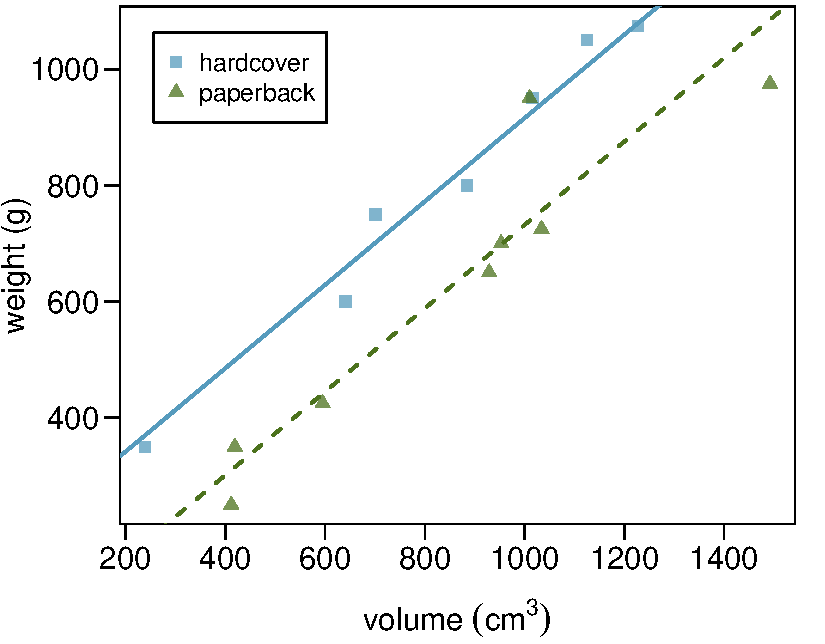
\includegraphics[width=0.8\textwidth]{plots/weight_volume_cover_lines}
\end{center}

\end{frame}

%%%%%%%%%%%%%%%%%%%%%%%%%%%%%%%%%%%

\begin{frame}
\frametitle{Interpretation of the regression coefficients}

{\small
\begin{center}
\begin{tabular}{rrrrr}
  \hline
 & Estimate & Std. Error & t value & Pr($>$$|$t$|$) \\ 
  \hline
(Intercept) & 197.96 & 59.19 & 3.34 & 0.01 \\ 
  volume & 0.72 & 0.06 & 11.67 & 0.00 \\ 
  cover:pb & -184.05 & 40.49 & -4.55 & 0.00 \\ 
   \hline
\end{tabular}
\end{center}
}

\pause

\begin{itemize}

\item $\beta_1$: \pause \underline{All else held constant}, books that are 1 more cubic centimeter in volume tend to weigh about 0.72 grams more, on average.

\pause

\item $\beta_2$: \pause \underline{All else held constant}, the model predicts that paperback books weigh 184 grams lower than hardcover books, on average.

\pause

\item $\beta_0$: \pause Hardcover books with no volume are expected on average to weigh 198 grams. \pause
\begin{itemize}
\item \pause Obviously, the intercept does not make sense in the context.
\end{itemize}

\end{itemize}

\end{frame}

%%%%%%%%%%%%%%%%%%%%%%%%%%%%%%%%%%%

\begin{frame}
\frametitle{Prediction}

Which of the following is the correct calculation for the predicted weight of a paperback book that is 600 cm$^3$?

{\small
\begin{center}
\begin{tabular}{rrrrr}
  \hline
 & Estimate & Std. Error & t value & Pr($>$$|$t$|$) \\ 
  \hline
(Intercept) & 197.96 & 59.19 & 3.34 & 0.01 \\ 
  volume & 0.72 & 0.06 & 11.67 & 0.00 \\ 
  cover:pb & -184.05 & 40.49 & -4.55 & 0.00 \\ 
   \hline
\end{tabular}
\end{center}
}

\begin{enumerate}[(a)]
\item 197.96 + 0.72 * 600 - 184.05 * 1 \only<2>{{\color{blue}{~$= 445.91$ grams}}}
\item 184.05 + 0.72 * 600 - 197.96 * 1
\item 197.96 + 0.72 * 600 - 184.05 * 0
\item 197.96 + 0.72 * 1 - 184.05 * 600
\end{enumerate}

\end{frame}



\begin{frame}{6.2 General linear model in matrix terms}
Response vector:
$$
\mathbf{Y}=\begin{bmatrix}
Y_1\\Y_2\\\vdots\\Y_n
\end{bmatrix}
$$

\pause Design matrix: 
$$
\mathbf{X}=\begin{bmatrix}
1 & x_{11} & x_{12} & \cdots & x_{1k}\\
1 & x_{21} & x_{22} & \cdots & x_{2k}\\
\vdots & \vdots & \vdots & \ddots & \vdots\\
1 & x_{n1} & x_{n2} & \cdots & x_{nk}
\end{bmatrix}
$$
The first column is a place-holder for the intercept term. 

\pause What does each column represent? \pause What does each row represent?
\end{frame}

\begin{frame}{General linear model in matrix terms}
(Unknown) regression coefficients:
$$\boldsymbol\beta=\begin{bmatrix}
\beta_0\\\beta_1\\\vdots\\\beta_k
\end{bmatrix}$$

(Unobserved) error vector:
$$
\boldsymbol\epsilon=\begin{bmatrix}
\epsilon_1\\\epsilon_2\\\vdots\\\epsilon_n
\end{bmatrix}
$$
\end{frame}

\begin{frame}{General linear model in matrix terms}
The general linear model is written in matrix terms as
$$
\mathbf{Y}=\underbrace{\begin{bmatrix}
Y_1\\Y_2\\\vdots\\Y_n
\end{bmatrix}}_{n\times1}=\underbrace{\begin{bmatrix}
1 & x_{11} & x_{12} & \cdots & x_{1k}\\
1 & x_{21} & x_{22} & \cdots & x_{2k}\\
\vdots & \vdots & \vdots & \ddots & \vdots\\
1 & x_{n1} & x_{n2} & \cdots & x_{nk} 
\end{bmatrix}}_{n\times p} \underbrace{\begin{bmatrix}
\beta_0\\\beta_1\\\vdots\\\beta_k
\end{bmatrix}}_{p\times1} + \underbrace{\begin{bmatrix}
\epsilon_1\\\epsilon_2\\\vdots\\\epsilon_n
\end{bmatrix}}_{n\times1},
$$
where $p=k+1$, or in short as
$$
\mathbf{Y}=\mathbf{X}\boldsymbol{\beta}+\boldmath{\epsilon}.
$$
\end{frame}

\begin{frame}{General linear model in matrix terms}
Minimal assumptions about the random error vector $\boldsymbol\epsilon$ are
$$
\E[\boldsymbol\epsilon]=\mathbf{0}\quad\text{and}\quad\Cov[\boldsymbol\epsilon]=\sigma^2\mathbf{I}_n,
$$
where $\mathbf{I}_n$ is the $n\times n$ identity matrix.
\vspace{10pt}

\pause In general, we will require more and assume
$$
\boldsymbol\epsilon\sim\mathcal{N}_n(\mathbf{0}, \sigma^2\mathbf{I}_n).
$$
\pause This allows us to construct $t$ and $F$ tests, obtain confidence intervals, etc.

\end{frame}

\begin{frame}{Fitting the model}
Estimating $\boldsymbol\beta=(\beta_0,\beta_1,\ldots,\beta_k)^\top$
\vspace{10pt}

\pause Recall the least-squares method:
$$
Q(\boldsymbol\beta)=\sum_{i=1}^n[Y_i-(\beta_0+\beta_1 x_{i1}+\ldots+\beta_k x_{ik})]^2\longrightarrow\min_{\boldsymbol\beta}
$$
\pause Using matrix calculus we can show that the LSEs are
$$
\mathbf{b}=\begin{bmatrix}
b_0\\b_1\\\vdots\\b_k
\end{bmatrix}=(\mathbf{X}^\top\mathbf{X})^{-1}\mathbf{X}^\top\mathbf{Y}
$$
\pause These are also MLEs.
\end{frame}

\begin{frame}{Fitted values, residuals, and hat matrix}
The \textit{fitted values} are 
$$
\hat{\mathbf{Y}}=\begin{bmatrix}
\hat{Y}_1\\\hat{Y}_2\\\vdots\\\hat{Y}_n
\end{bmatrix}=\mathbf{Xb}\pause=\underbrace{[\mathbf{X}(\mathbf{X}^\top\mathbf{X})^{-1}\mathbf{X}^\top]}_{\text{projection matrix}}\mathbf{Y} = \mathbf{HY}.
$$
\pause The \textit{residuals} are 
$$
\mathbf{e}=\begin{bmatrix}
e_1\\e_2\\\vdots\\e_n
\end{bmatrix}\pause=\mathbf{Y}-\hat{\mathbf{Y}}\pause=\mathbf{Y}-\mathbf{Xb}\pause=[\mathbf{I}_n-\mathbf{X}(\mathbf{X}^\top\mathbf{X})^{-1}\mathbf{X}^\top]\mathbf{Y}.
$$\pause
$\mathbf{H}=\mathbf{X}(\mathbf{X}^\top\mathbf{X})^{-1}\mathbf{X}^\top$ is called the \textbf{hat matrix} or \textbf{projection matrix}. We'll use it shortly when we talk about diagnostics. Notice that $\mathbf{e}=(\mathbf{I}-\mathbf{H})\mathbf{Y}$.
\end{frame}

\begin{frame}{Example: Dwayne Studios}


In the \textbf{Dwayne Portrait Studio data,} we have
$$
\mathbf{b}=\begin{bmatrix}
b_0\\b_1\\b_2
\end{bmatrix}=\begin{bmatrix}
-68.857\\1.455\\9.366
\end{bmatrix},
$$
\pause so the fitted regression line is
$$
\hat{Y}=-68.857+1.455\cdot{x_1} + 9.366\cdot {x_2},
$$
\pause where $x_1$ is \# children in thousands, $x_2$ is income in thousand \$'s.
\begin{itemize}
\item \pause $b_1$: \pause For 1000  increase in number of children, mean sales increase by \$1,455 holding per capita income constant.
\item \pause $b_2$: \pause For each \$1000 increase in per capita income, mean sales increase by \$9,366, holding the number of children constant.
\end{itemize}
\end{frame}


\begin{frame}{Partitioning SST}
Recall the decomposition
$$
\underbrace{\sum_{i=1}^n (Y_i-\bar{Y})^2}_{\text{SST}}=\underbrace{\sum_{i=1}^n (Y_i-\hat{Y}_i)^2}_{\text{SSE}}+\underbrace{\sum_{i=1}^n(\hat{Y}_i-\bar{Y})^2}_{\text{SSR}}
$$
\onslide<2->{Notice that}
\begin{align*}
\onslide<2->{\text{SSE}&=(\mathbf{Y}-\hat{\mathbf{Y}})^\top(\mathbf{Y}-\hat{\mathbf{Y}})=\mathbf{Y}^\top(\mathbf{I}-{\mathbf{H}})^\top(\mathbf{I}-{\mathbf{H}})\mathbf{Y}=\mathbf{Y}^\top(\mathbf{I}-\mathbf{H})\mathbf{Y}\\}
\onslide<3->{\text{SSR}&=(\hat{\mathbf{Y}}-\bar{\mathbf{Y}})^\top(\hat{\mathbf{Y}}-\bar{\mathbf{Y}})=\mathbf{Y}^\top\left(\mathbf{H}-\frac1n\mathbf{J}\right)^\top\left(\mathbf{H}-\frac1n\mathbf{J}\right)\mathbf{Y}\\
&=\mathbf{Y}^\top\left(\mathbf{H}-\frac1n\mathbf{J}\right)\mathbf{Y}}
\end{align*}
\onslide<4->{where $\frac1n\mathbf{J}=\mathbf{1}(\mathbf{1}^\top\mathbf{1})^{-1}\mathbf{1}^\top$}\onslide<5->{, and we used symmetry and idempotence of $\mathbf{I}-\mathbf{H}$ and $\mathbf{H}-\frac1n\mathbf{J}$ (Ch 5).}
\end{frame}

\begin{frame}{Distribution of SSE}
\begin{theorem}
$\frac{\text{SSE}}{\sigma^2}\sim\chi^2_{n-p}$
\end{theorem}
\begin{proof}
$\mathbf{Y}\sim\mathcal{N}_n(\mathbf{X}\boldsymbol\beta,\sigma^2\mathbf{I})$\pause\quad$\Rightarrow$\quad$\sigma^{-1}\mathbf{Y}\sim\mathcal{N}_n(\sigma^{-1}\mathbf{X}\boldsymbol\beta,\mathbf{I})$. \pause Hence, 
\begin{align*}
\onslide<3->{\frac{\text{SSE}}{\sigma^2}&=(\sigma^{-1}\mathbf{Y})^\top(\mathbf{I}-\mathbf{H})(\sigma^{-1}\mathbf{Y})\pause}\onslide<4->{\sim\chi^2_{\rank[\mathbf{I}-\mathbf{H}]}(\lambda),\\}
\onslide<5->{\text{where\quad }\rank[\mathbf{I}-\mathbf{H}]&=\trace[\mathbf{I}-\mathbf{H}]}\onslide<6->{=\trace[\mathbf{I}-\mathbf{X}(\mathbf{X}^\top\mathbf{X})^{-1}\mathbf{X}^\top]\\}
\onslide<7->{&=\trace\mathbf{I}-\trace[\mathbf{X}(\mathbf{X}^\top\mathbf{X})^{-1}\mathbf{X}^\top]\\}
\onslide<8->{&=n-\trace[(\mathbf{X}^\top\mathbf{X})^{-1}\mathbf{X}^\top\mathbf{X}]}\onslide<9->{=n-p,\\}
\onslide<10->{\text{and\quad }\lambda&=(\sigma^{-1}\mathbf{X}\boldsymbol\beta)^\top(\mathbf{I}-\mathbf{H})(\sigma^{-1}\mathbf{X}\boldsymbol\beta)\\}
\onslide<11->{&=\frac1{\sigma^2}\boldsymbol\beta^\top\mathbf{X}^\top[\mathbf{I}-\mathbf{X}(\mathbf{X}^\top\mathbf{X})^{-1}\mathbf{X}^\top]\mathbf{X}\boldsymbol\beta\\}
\onslide<12->{&=\frac{1}{\sigma^2}\boldsymbol\beta^\top[\mathbf{X}^\top\mathbf{X}-\mathbf{X}^\top\mathbf{X}(\mathbf{X}^\top\mathbf{X})^{-1}\mathbf{X}^\top\mathbf{X}]\boldsymbol\beta}\onslide<13->{=0}
\end{align*}
\end{proof}
\end{frame}


\begin{frame}{Some properties of the hat matrix}
\begin{lemma}
$\mathbf{H}\mathbf{1}=\mathbf{1}$
\end{lemma}
\begin{proof}
\begin{align*}
\onslide<2->{\mathbf{X}(\mathbf{X}^\top\mathbf{X})^{-1}\mathbf{X}^\top\mathbf{X}&=\mathbf{X}\\}
\onslide<3->{\mathbf{X}(\mathbf{X}^\top\mathbf{X})^{-1}\mathbf{X}^\top\begin{bmatrix}\mathbf{1} & \mathbf{\tilde{X}}\end{bmatrix}&=\begin{bmatrix}\mathbf{1} & \mathbf{\tilde{X}}\end{bmatrix}\\}
\onslide<4->{\begin{bmatrix}\mathbf{X}(\mathbf{X}^\top\mathbf{X})^{-1}\mathbf{X}^\top\mathbf{1} & \mathbf{X}(\mathbf{X}^\top\mathbf{X})^{-1}\mathbf{X}^\top\mathbf{\tilde{X}}\end{bmatrix}&=\begin{bmatrix}\mathbf{1} & \mathbf{\tilde{X}}\end{bmatrix}}
\end{align*}
\onslide<5->{Hence, $\mathbf{H1}=\mathbf{X}(\mathbf{X}^\top\mathbf{X})^{-1}\mathbf{X}^\top\mathbf{1}=\mathbf{1}$.}
\end{proof}
\begin{remark}
\onslide<6->{$\mathbf{H}\mathbf{\tilde{X}}=\mathbf{\tilde{X}}$}\onslide<7->{, $\mathbf{1}^\top\mathbf{H}=\mathbf{1}^\top$}\onslide<8->{, $\mathbf{\tilde{X}}^\top\mathbf{H}=\mathbf{\tilde{X}}^\top$}
\end{remark}
\end{frame}

\iffalse
\begin{proof}
$\mathbf{1}^\top\mathbf{H}=\mathbf{1}^\top\mathbf{X}(\mathbf{X}^\top\mathbf{X})^{-1}\mathbf{X}^\top=\mathbf{1}^\top\begin{bmatrix}\mathbf{1} & \mathbf{\tilde{X}}\end{bmatrix}\left(\begin{bmatrix}\mathbf{1}^\top\\\mathbf{\tilde{X}}^\top\end{bmatrix}\begin{bmatrix}\mathbf{1} & \mathbf{\tilde{X}}\end{bmatrix}\right)^{-1}\begin{bmatrix}\mathbf{1}^\top\\\mathbf{\tilde{X}}^\top\end{bmatrix}$

$\left(\begin{bmatrix}\mathbf{1}^\top\\\mathbf{\tilde{X}}^\top\end{bmatrix}\begin{bmatrix}\mathbf{1} & \mathbf{\tilde{X}}\end{bmatrix}\right)^{-1}=\begin{bmatrix}
\mathbf{1}^\top\mathbf{1} & \mathbf{1}^\top\mathbf{\tilde{X}}\\
\mathbf{\tilde{X}}^\top\mathbf{1} & \mathbf{\tilde{X}}^\top\mathbf{\tilde{X}}
\end{bmatrix}^{-1}=\begin{bmatrix}
n & \mathbf{1}^\top\mathbf{\tilde{X}}\\
\mathbf{\tilde{X}}^\top\mathbf{1} & \mathbf{\tilde{X}}^\top\mathbf{\tilde{X}}
\end{bmatrix}^{-1}=\begin{bmatrix}
(n-\mathbf{1}^\top\mathbf{\tilde{X}}(\mathbf{\tilde{X}}^\top\mathbf{\tilde{X}})^{-1}\mathbf{\tilde{X}}^\top\mathbf{1})^{-1} & \mathbf{0}\\
\mathbf{0} & (\mathbf{\tilde{X}}^\top\mathbf{\tilde{X}}-\mathbf{\tilde{X}}^\top\mathbf{1}n^{-1}\mathbf{1}^\top\mathbf{\tilde{X}})^{-1}\end{bmatrix}\begin{bmatrix}1 & -\mathbf{1}^\top\mathbf{\tilde{X}}(\mathbf{\tilde{X}}^\top\mathbf{\tilde{X}})^{-1}\\
-\mathbf{\tilde{X}}^\top\mathbf{1}n^{-1} & \mathbf{I}
\end{bmatrix}$

$\mathbf{1}^\top\mathbf{H}=\mathbf{1}^\top\begin{bmatrix}
\mathbf{1}(n-\mathbf{1}^\top\mathbf{\tilde{X}}(\mathbf{\tilde{X}}^\top\mathbf{\tilde{X}})^{-1}\mathbf{\tilde{X}}^\top\mathbf{1})^{-1} &  \mathbf{\tilde{X}}(\mathbf{\tilde{X}}^\top\mathbf{\tilde{X}}-\mathbf{\tilde{X}}^\top\mathbf{1}n^{-1}\mathbf{1}^\top\mathbf{\tilde{X}})^{-1}\end{bmatrix}\begin{bmatrix}\mathbf{1}^\top-\mathbf{1}^\top\mathbf{\tilde{X}}(\mathbf{\tilde{X}}^\top\mathbf{\tilde{X}})^{-1}\mathbf{\tilde{X}}^\top \\
-\mathbf{\tilde{X}}^\top\mathbf{1}n^{-1}\mathbf{1}^\top+\mathbf{\tilde{X}}^\top
\end{bmatrix}=\begin{bmatrix}
n(n-\mathbf{1}^\top\mathbf{\tilde{X}}(\mathbf{\tilde{X}}^\top\mathbf{\tilde{X}})^{-1}\mathbf{\tilde{X}}^\top\mathbf{1})^{-1} &  \mathbf{1}^\top\mathbf{\tilde{X}}(\mathbf{\tilde{X}}^\top\mathbf{\tilde{X}}-\mathbf{\tilde{X}}^\top\mathbf{1}n^{-1}\mathbf{1}^\top\mathbf{\tilde{X}})^{-1}\end{bmatrix}\begin{bmatrix}\mathbf{1}^\top-\mathbf{1}^\top\mathbf{\tilde{X}}(\mathbf{\tilde{X}}^\top\mathbf{\tilde{X}})^{-1}\mathbf{\tilde{X}}^\top \\
-\mathbf{\tilde{X}}^\top\mathbf{1}n^{-1}\mathbf{1}^\top+\mathbf{\tilde{X}}^\top
\end{bmatrix}$

$(\mathbf{1}^\top(\mathbf{I}-\mathbf{P})\mathbf{1})^{-1}\mathbf{1}^\top(\mathbf{I}-\mathbf{P})+\mathbf{1}^\top\mathbf{\tilde{X}}(\mathbf{\tilde{X}}^\top\mathbf{\tilde{X}}-\mathbf{\tilde{X}}^\top\mathbf{1}n^{-1}\mathbf{1}^\top\mathbf{\tilde{X}})^{-1}(\mathbf{\tilde{X}}^\top-\mathbf{\tilde{X}}^\top\mathbf{1}n^{-1}\mathbf{1}^\top)$
\end{proof}
\fi


\begin{frame}{Distribution of SSR}
\begin{theorem}
$\frac{\text{SSR}}{\sigma^2}\sim\chi^2_{p-1}(\lambda)$ \pause with $\lambda=\frac{1}{\sigma^2}\boldsymbol{\tilde\beta}^\top\mathbf{\bar{X}}^\top\mathbf{\bar{X}}\boldsymbol{\tilde\beta}$, \pause where
$$
\boldsymbol{\tilde\beta}=\begin{bmatrix}
\beta_1\\
\beta_2\\
\vdots\\
\beta_k
\end{bmatrix},\pause\quad\mathbf{\bar{X}}=\begin{bmatrix}
x_{11}-\bar{x}_1 & x_{12}-\bar{x}_2 & \cdots & x_{1k}-\bar{x}_k\\
x_{21}-\bar{x}_1 & x_{22}-\bar{x}_2 & \cdots & x_{2k}-\bar{x}_k\\
\vdots & \vdots & \ddots & \vdots\\
x_{n1}-\bar{x}_1 & x_{n2}-\bar{x}_2 & \cdots & x_{nk}-\bar{x}_k
\end{bmatrix}
$$
\pause and $\bar{x}_j:=\frac1n\sum_{i=1}^n x_{ij}$ is the average value of the $j^\text{th}$ predictor.
\end{theorem}
\begin{block}{Proof.}
\pause The proof is analogous to the case of $k=1$. \pause Let's focus on $\lambda$. \pause
Let $\mathbf{\tilde{X}}=\begin{bmatrix}x_{11} & \cdots & x_{1k}\\\vdots & \ddots & \vdots\\x_{n1} & \cdots &  x_{nk}\end{bmatrix}$, \pause  then $\mathbf{X}\boldsymbol\beta=\begin{bmatrix}\mathbf{1} & \mathbf{\tilde{X}}\end{bmatrix}\begin{bmatrix}\beta_0\\\boldsymbol{\tilde\beta}\end{bmatrix}=\beta_0\mathbf{1}+\mathbf{\tilde{X}}\boldsymbol{\tilde\beta}$
\end{block}
\end{frame}


\begin{frame}{Distribution of SSR}
\begin{proof}[Proof (cont'd)]
Since $\frac{\text{SSR}}{\sigma^2}=(\frac1\sigma\mathbf{Y})^\top\left(\mathbf{H}-\frac1n\mathbf{J}\right)(\frac1\sigma\mathbf{Y})$ and $\frac1\sigma\mathbf{Y}\sim\mathcal{N}_n(\frac1\sigma\mathbf{X}\boldsymbol\beta,\mathbf{I})$,
\begin{align*}
\onslide<2->{\lambda&=\frac1{\sigma^2}\boldsymbol\beta^\top\mathbf{X}^\top[\mathbf{X}(\mathbf{X}^\top\mathbf{X})^{-1}\mathbf{X}^\top-\mathbf{1}(\mathbf{1}^\top\mathbf{1})^{-1}\mathbf{1}^\top]\mathbf{X}\boldsymbol\beta\\}
\onslide<3->{&=\frac{1}{\sigma^2}\begin{bmatrix}\beta_0 & \boldsymbol{\tilde\beta}^\top\end{bmatrix}\begin{bmatrix}\mathbf{1}^\top\\\mathbf{\tilde{X}}^\top\end{bmatrix}[\mathbf{X}(\mathbf{X}^\top\mathbf{X})^{-1}\mathbf{X}^\top-\mathbf{1}(\mathbf{1}^\top\mathbf{1})^{-1}\mathbf{1}^\top]\begin{bmatrix}\mathbf{1} & \mathbf{\tilde{X}}\end{bmatrix}\begin{bmatrix}\beta_0\\\boldsymbol{\tilde\beta}\end{bmatrix}\\}
\onslide<4->{&=\frac{1}{\sigma^2}\begin{bmatrix}\beta_0 & \boldsymbol{\tilde\beta}^\top\end{bmatrix}\begin{bmatrix}\mathbf{1}^\top\mathbf{X}(\mathbf{X}^\top\mathbf{X})^{-1}\mathbf{X}^\top-\mathbf{1}^\top\mathbf{1}(\mathbf{1}^\top\mathbf{1})^{-1}\mathbf{1}^\top\\\mathbf{\tilde{X}}^\top\mathbf{X}(\mathbf{X}^\top\mathbf{X})^{-1}\mathbf{X}^\top-\mathbf{\tilde{X}}^\top\mathbf{1}(\mathbf{1}^\top\mathbf{1})^{-1}\mathbf{1}^\top\end{bmatrix}\begin{bmatrix}\mathbf{1} & \mathbf{\tilde{X}}\end{bmatrix}\begin{bmatrix}\beta_0\\\boldsymbol{\tilde\beta}\end{bmatrix}\\}
\onslide<5->{&=\frac{1}{\sigma^2}\begin{bmatrix}\beta_0 & \boldsymbol{\tilde\beta}^\top\end{bmatrix}\begin{bmatrix}\mathbf{1}^\top-\mathbf{1}^\top\\\mathbf{\tilde{X}}^\top-\mathbf{\tilde{X}}^\top\mathbf{1}(\mathbf{1}^\top\mathbf{1})^{-1}\mathbf{1}^\top\end{bmatrix}\begin{bmatrix}\mathbf{1} & \mathbf{\tilde{X}}\end{bmatrix}\begin{bmatrix}\beta_0\\\boldsymbol{\tilde\beta}\end{bmatrix}\\}
\onslide<6->{&=\frac{1}{\sigma^2}\begin{bmatrix}\beta_0 & \boldsymbol{\tilde\beta}^\top\end{bmatrix}\begin{bmatrix}0 & \mathbf{0}^\top\\\mathbf{0} & \mathbf{\tilde{X}}^\top\mathbf{\tilde{X}}-\mathbf{\tilde{X}}^\top\mathbf{1}(\mathbf{1}^\top\mathbf{1})^{-1}\mathbf{1}^\top\mathbf{\tilde{X}}\end{bmatrix}\begin{bmatrix}\beta_0\\\boldsymbol{\tilde\beta}\end{bmatrix}\\}
\onslide<7->{&=\frac{1}{\sigma^2} \boldsymbol{\tilde\beta}^\top[\mathbf{\tilde{X}}^\top\mathbf{\tilde{X}}-\mathbf{\tilde{X}}^\top\mathbf{1}(\mathbf{1}^\top\mathbf{1})^{-1}\mathbf{1}^\top\mathbf{\tilde{X}}]\boldsymbol{\tilde\beta}}\onslide<8->{=\frac{1}{\sigma^2}\boldsymbol{\tilde\beta}^\top\mathbf{\bar{X}}^\top\mathbf{\bar{X}}\boldsymbol{\tilde\beta}}
\end{align*}
\end{proof}    
\end{frame}


\begin{frame}{Means of SSE and SSR}
\begin{theorem}
Let $\text{MSE}:=\frac{\text{SSE}}{n-p}$, then $\E[\text{MSE}]=\sigma^2$.
\end{theorem}
\begin{proof}
\pause $\frac{\text{SSE}}{\sigma^2}\sim\chi^2_{n-p}$\pause\quad$\Rightarrow$\quad$\E\left[\frac{\text{SSE}}{\sigma^2}\right]=n-p$\pause\quad$\Rightarrow$\quad$\E\left[\frac{\text{SSE}}{n-p}\right]=\sigma^2$
\end{proof}
\pause\begin{theorem}
Let $\text{MSR}:=\frac{\text{SSR}}{p-1}$, then $\E[\text{MSR}]=\sigma^2+\frac{1}{p-1}\boldsymbol{\tilde\beta}^\top\mathbf{\bar{X}}^\top\mathbf{\bar{X}}\boldsymbol{\tilde\beta}$
\end{theorem}
\begin{proof}
\vspace{-20pt}
\pause\begin{align*}
\onslide<7->{&\frac{\text{SSR}}{\sigma^2}\sim\chi^2_{p-1}(\lambda)\text{ with }\lambda=\frac{1}{\sigma^2}\boldsymbol{\tilde\beta}^\top\mathbf{\bar{X}}^\top\mathbf{\bar{X}}\boldsymbol{\tilde\beta}\\}
\onslide<8->{&\Rightarrow\quad\E\left[\frac{\text{SSR}}{\sigma^2}\right]=p-1+\frac{1}{\sigma^2}\boldsymbol{\tilde\beta}^\top\mathbf{\bar{X}}^\top\mathbf{\bar{X}}\boldsymbol{\tilde\beta}\\}
\onslide<9->{&\Rightarrow\quad\E\left[\text{MSR}\right]=\sigma^2+\frac{1}{p-1}\boldsymbol{\tilde\beta}^\top\mathbf{\bar{X}}^\top\mathbf{\bar{X}}\boldsymbol{\tilde\beta}}
\end{align*}
\end{proof}
\end{frame}


\begin{frame}{Analysis of variance}
In multiple regression we can decompose the total sum of squares into the SSR and SSE pieces. \pause The table is now
\vspace{5pt}

\begin{center}
\begin{footnotesize}
\begin{tabular}{l r c c c}
Source & SS & df & MS & $\E[MS]$\\
\hline
Regression & $\mathrm{SSR}=\sum(\hat{Y}_i-\bar{Y})^2$ & ${\color{blue}p-1}$ & $\frac{\rm SSR}{p-1}$ & $\sigma^2+{\text{QF}}$\\
Error & $\mathrm{SSE}=\sum(Y_i-\hat{Y})^2$ & ${\color{blue}n-p}$ & $\frac{\rm SSE}{n-p}$ & $\sigma^2$\\
\hline
Total & $\mathrm{SST}=\sum(Y_i-\bar{Y})^2$ & $n-1$
\end{tabular}
\end{footnotesize}
\end{center}

where $p=k+1$.
\vspace{10pt}

\pause Here, QF stands for ``quadratic form'' and is given by
$$
\text{QF}=\frac{1}{p-1}\boldsymbol{\tilde\beta}^\top\mathbf{\bar{X}}^\top\mathbf{\bar{X}}\boldsymbol{\tilde\beta}=\frac1k\sum_{j=1}^k\sum_{s=1}^k\beta_j\beta_s\sum_{i=1}^n(x_{ij}-\bar{x}_j)(x_{is}-\bar{x}_s)\ge0.
$$
\pause Note that $\text{QF}=0$\quad $\Leftrightarrow$\quad $\beta_1=\beta_2=\ldots=\beta_k=0$.
\end{frame}

\begin{frame}{Overall $F$-test for a regression relationship (p.~226)}
In multiple regression, our $F$-test based on $F^\ast=\frac{\rm MSR}{\rm MSE}$ tests whether the \textit{entire set} of predictors $x_1,\ldots,x_k$ explains a significant amount of variation in $Y$.
\vspace{10pt}

\pause If MSR $\approx$ MSE, there's no evidence that \textit{any} of the predictors are useful. If MSR $\gg$ MSE, then \textit{some} of them are useful.
\vspace{10pt}

\pause Formally, we test
$$
\mathrm{H}_0: \beta_1=\beta_2=\ldots=\beta_k=0
$$
\pause versus
$$
\mathrm{H}_a: \text{ at least one  }\beta_j\ne0.
$$
\pause If $F^\ast>F_{p-1,n-p,1-\alpha}$, we reject $\mathrm{H}_0$ and conclude that \textit{something} is going on, there is \textit{some} relationship between one or more of the $x_1,\ldots,x_k$ and $Y$. {\sc R} provides a p-value for this test.
\end{frame}

\begin{frame}{$R^2$ in case of multiple regression}
The \textbf{coefficient of multiple determination} is
$$
R^2=\frac{\rm SSR}{\rm SST}=1-\frac{\rm SSE}{\rm SST}.
$$
measures the proportion of sample variation in $Y$ explained by its \textit{linear} relationship with the predictors $x_1,\ldots,x_k$. As before, $0\le R^2\le1$.
\vspace{10pt}

\pause When we add a predictor to the model $R^2$ can only increase. (Why?)
\vspace{10pt}

\pause The \textbf{adjusted $R^2$}
$$
R_a^2=1-\frac{\mathrm{SSE}/(n-p)}{\mathrm{SST}/(n-1)}
$$
accounts for the number of predictors in the model. It may decrease when we add useless predictors to the model.
\end{frame}

\begin{frame}[fragile]{Dwayne Studio Regression Output}{\url{https://github.com/zh3nis/MATH440/blob/main/chp06/mlr.R}}
\begin{footnotesize}
\begin{verbatim}
> m = lm(sales ~ children + income, data=dwayne)
> summary(m)
...
Multiple R-squared:  0.9167,	Adjusted R-squared:  0.9075 
F-statistic:  99.1 on 2 and 18 DF,  p-value: 1.921e-10

> anova(m)
Analysis of Variance Table

Response: sales
          Df  Sum Sq Mean Sq  F value   Pr(>F)    
children   1 23371.8 23371.8 192.8962 4.64e-11 ***
income     1   643.5   643.5   5.3108  0.03332 *  
Residuals 18  2180.9   121.2
\end{verbatim}
\end{footnotesize}

Conclusions?

\pause
We reject $H_0:\beta_1=\beta_2=0$ at any reasonable significance level $\alpha$. About 92\% of the total variability in the data is explained by the linear regression model.
\end{frame}

\begin{frame}{Inference about individual regression parameters}
The overall $F$-test concerns the \textit{entire set} of predictors $x_1,\ldots,x_k$.
\vspace{10pt}

\pause If the $F$-test is significant, we will want to determine \textit{which} of the individual predictors contribute significantly to the model.
\vspace{10pt}

\pause We will talk about this shortly, but the main methods are forward selection, backwards elimination, stepwise procedures, $C_p$, $R_a^2$, LASSO, etc.
\end{frame}

\begin{frame}{Mean and covariance matrix of a vector}
\structure{Recall}: If $\mathbf{Y}$ is a random vector, then its \alert{expected value} is also a vector
$$
\E[\mathbf{Y}]=\begin{bmatrix}
\E[Y_1]\\\E[Y_2]\\\vdots\\\E[Y_n]
\end{bmatrix}
$$
The random vector $\mathbf{Y}$ also has a \alert{covariance matrix}
$$
\Cov[\mathbf{Y}]=\begin{bmatrix}
\Cov[Y_1,Y_1] & \Cov[Y_1,Y_2] & \cdots & \Cov[Y_1,Y_n]\\
\Cov[Y_2,Y_1] & \Cov[Y_2,Y_2] & \cdots & \Cov[Y_2,Y_n]\\
\vdots & \vdots & \ddots & \vdots\\
\Cov[Y_n,Y_1] & \Cov[Y_n, Y_2] & \cdots & \Cov[Y_n, Y_n].
\end{bmatrix}
$$
\end{frame}

\begin{frame}{Multivariate normal}
The \textbf{multivariate normal} density is given by
$$
f(\mathbf{y})=|2\pi\mathbf{\Sigma}|^{-1/2}\exp\{-0.5(\mathbf{y}-\boldsymbol\mu)'\mathbf\Sigma^{-1}(\mathbf{y}-\boldsymbol\mu)\},$$
where $\mathbf{y}\in\mathbb{R}^n$. We write
$$
\mathbf{Y}\sim\mathcal{N}_n(\boldsymbol\mu, \mathbf\Sigma).
$$
Then $\E[\mathbf{Y}]=\boldsymbol\mu$ and $\Cov[\mathbf{Y}]=\mathbf\Sigma$.
\vspace{10pt}

For the general linear model,
$$
\mathbf{Y}\sim\mathcal{N}_n(\mathbf{X}\boldsymbol\beta,\sigma^2\mathbf{I}_n).
$$
\end{frame}

\begin{frame}{Error vector}
Note that along the diagonal of $\Cov[\mathbf{Y}]$, $\Cov[Y_i, Y_i]=\Var[Y_i]$.
\vspace{10pt}

For the general linear model,
$$
\E[\boldsymbol\epsilon]=\mathbf{0}=\begin{bmatrix}
0\\0\\\vdots\\0
\end{bmatrix},
$$

$$
\Cov[\boldsymbol\epsilon]=\sigma^2\mathbf{I}_n=\begin{bmatrix}
\sigma^2 & 0 & \cdots & 0\\
0 & \sigma^2 & \cdots & 0\\
\vdots & \vdots & \ddots & \vdots\\
0 & 0 & \cdots & \sigma^2
\end{bmatrix}.
$$
\end{frame}

\begin{frame}{Inference for $\boldsymbol\beta$}
$$
\Cov[\mathbf{Y}]=\Cov[\underbrace{\mathbf{X}\boldsymbol\beta}_{\text{fixed}}+\underbrace{\boldsymbol\epsilon}_{\text{random}}]=\Cov[\boldsymbol\epsilon]
$$

\hrulefill

Fact: If $\mathbf{A}$ is a constant matrix, $\mathbf{a}$ is a constant vector, and $\mathbf{Y}$ is any random vector, then
$$
\E[\mathbf{AY}+\mathbf{a}]=\mathbf{A}\E[\mathbf{Y}]+\mathbf{a},
$$
$$
\Cov[\mathbf{AY+a}]=\mathbf{A}\Cov[\mathbf{Y}]\mathbf{A}^\top.
$$
\end{frame}

\begin{frame}{Back to the general linear model}
For $\hat{\mathbf{Y}}=\mathbf{HY}$,
\pause $$
\E[\hat{\mathbf{Y}}]=\mathbf{H}\E[\mathbf{Y}]=\mathbf{HX}\boldsymbol{\beta}=\mathbf{X(X'X)}^{-1}\mathbf{X'X}\boldsymbol{\beta}=\mathbf{X}\boldsymbol{\beta}.
$$
\pause $$
\Cov[\hat{\mathbf{Y}}]=\mathbf{H}\Cov[\mathbf{Y}]\mathbf{H'}=\sigma^2\mathbf{H},
$$
\pause since $\mathbf{HH'}=\mathbf{H}$ (property of a {\it projection matrix}).

\pause For $\mathbf{e}=(\mathbf{I}_n-\mathbf{H})\mathbf{Y}$,
\pause $$
\E[\mathbf{e}]=(\mathbf{I}_n-\mathbf{H})\E[\mathbf{Y}]=(\mathbf{I}_n-\mathbf{H})\mathbf{X}\boldsymbol\beta=\mathbf{X}\boldsymbol\beta=\mathbf{X}\boldsymbol\beta-\mathbf{HX}\boldsymbol\beta=\mathbf{0},
$$
\pause as $\mathbf{HX}=\mathbf{X}$ (projection matrix again).
\pause $$
\Cov[\mathbf{e}]=(\mathbf{I}_n-\mathbf{H})\Cov[\mathbf{Y}](\mathbf{I}_n-\mathbf{H})'=\sigma^2(\mathbf{I}_n-\mathbf{H}).
$$
(Why?)
\end{frame}

\begin{frame}{Mean and variance of $\mathbf{b}$}
Finally, $\mathbf{b}=(\mathbf{X'X})^{-1}\mathbf{X'Y}$ is {\it unbiased}
$$
\E[\mathbf{b}]=(\mathbf{X'X})^{-1}\mathbf{X}'\E[\mathbf{Y}]=(\mathbf{X'X})^{-1}\mathbf{X'X}\boldsymbol\beta=\boldsymbol\beta,
$$
and has covariance matrix
\begin{align*}
\Cov[\mathbf{b}]&=(\mathbf{X'X})^{-1}\mathbf{X}'\Cov[\mathbf{Y}][(\mathbf{X'X})^{-1}\mathbf{X'}]'\\
&=\sigma^2(\mathbf{X'X})^{-1}\mathbf{X}'[(\mathbf{X'X})^{-1}\mathbf{X}']'\\
&=\sigma^2(\mathbf{X'X})^{-1}\mathbf{X'X}(\mathbf{X'X})^{-1}\\
&=\sigma^2(\mathbf{X'X})^{-1}.
\end{align*}
Hence,
$$
\mathbf{b}\sim\mathcal{N}_p(\boldsymbol\beta, \sigma^2(\mathbf{X'X})^{-1}).
$$
\end{frame}

\begin{frame}{Table of regression effects}
From the previous slide, the $j$th estimated coefficient $\beta_j$,
$$
\Var[b_j]=\sigma^2 c_{jj},
$$
where $c_{jj}$ is the $j$th diagonal element of $(\mathbf{X'X})^{-1}$.\\~\\ 

As usually, we {\it estimate} the standard deviation of $b_j$ by $\s[b_j]=\sqrt{\mathrm{MSE}\cdot c_{jj}}$ yielding
$$
\frac{b_j-\beta_j}{\s[b_j]}\sim t_{n-p}
$$
{\bf Note:} {\sc R} gives each $\s[b_j]$ as well as $b_j$, $t^\ast_j=b_j/\s[b_j]$, and a $p$-value for testing each ${\rm H}_0:\beta_j=0$.
\end{frame}

\begin{frame}[fragile]{Dwayne output}
\begin{footnotesize}
\begin{verbatim}
Coefficients:
            Estimate Std. Error t value Pr(>|t|)    
(Intercept) -68.8571    60.0170  -1.147   0.2663    
children      1.4546     0.2118   6.868    2e-06 ***
income        9.3655     4.0640   2.305   0.0333 *  
---
Signif. codes:  0 ‘***’ 0.001 ‘**’ 0.01 ‘*’ 0.05 ‘.’ 0.1 ‘ ’ 1

Residual standard error: 11.01 on 18 degrees of freedom
Multiple R-squared:  0.9167,	Adjusted R-squared:  0.9075 
F-statistic:  99.1 on 2 and 18 DF,  p-value: 1.921e-10
\end{verbatim}
\end{footnotesize}
We reject ${\rm H}_0:\,\beta_1=0$ at the $\alpha=0.01$ level and ${\rm H}_0:\,\beta_2=0$ at the $\alpha=0.05$ level.
\end{frame}

\begin{frame}{Individual tests of ${\rm H}_0: \beta_j=0$}
\textbf{Note:} A test of ${\rm H}_0: \beta_j=0$ versus ${\rm H}_a: \beta_j=0$ -- available in the table of regression coefficients -- is a test of whether predictor $x_j$ is necessary in a model \textit{with the other remaining predictors included}.
\vspace{10pt}

For the Dwayne Studio Data:
\begin{itemize}
\item<2-> The {\sc R} summary gives us $F^\ast=\mathrm{MSR}/\mathrm{MSE}=99.10$ with associated p-value $<0.0001$ (it is actually $2\times10^{-10}$!). We strongly reject ${\rm H}_0: \beta_1=\beta_2=0$.
\item<3-> 95\% CI's are $(1.01, 1.90)$ for $\beta_1$ and $(0.83, 17.90)$ for $\beta_2$.
\item<4-> For example, we are 95\% confident that mean sales increases by \$1010 to \$1900 for every 1000 increase in kids 16 and under, holding income constant.
\item<5-> For ${\rm H}_0: \beta_1=0$ we get $p<0.0001$; for ${\rm H}_0: \beta_2=0$ we get $p=0.03$. Are people under 16 ($x_1$) and income ($x_2$) important in the model?
\end{itemize}
\end{frame}


\begin{frame}{CI for mean response and PI for new response}
Let's construct a CI for the mean response corresponding to a set of values
$$
\mathbf{x}_{\text{new}}=\begin{bmatrix}
1\\x_{\text{new},1}\\x_{\text{new},2}\\\vdots\\x_{\text{new},k}
\end{bmatrix}
$$
\pause We want to make inferences about
$$
\E[Y_{\text{new}}]=\mathbf{x}_\text{new}^\top\boldsymbol\beta=\beta_0+\beta_1 x_{\text{new},1}+\ldots+\beta_k x_{\text{new},k}.
$$
\end{frame}

\begin{frame}{CI for mean response and PI for new response}
\begin{itemize}
\item A point estimate is $\hat{Y}_\text{new}=\widehat{\E[Y_\text{new}]}=\mathbf{x}_\text{new}\mathbf{b}$.
\item\pause Then $\E[\hat{Y}_\text{new}]=\E[\mathbf{x}_\text{new}\mathbf{b}]=\mathbf{x}_\text{new}\E[\mathbf{b}]=\mathbf{x}_\text{new}\boldsymbol\beta$.
\item\pause Also, $\Var[\hat{Y}_\text{new}]=\Cov[\mathbf{x'}_\text{new}\mathbf{b}]=\mathbf{x'}_\text{new}\Cov[\mathbf{b}]\mathbf{x}_\text{new}=\sigma^2\mathbf{x'}_\text{new}(\mathbf{X'X})^{-1}\mathbf{x}_\text{new}$.
\end{itemize}
\pause So
\begin{itemize}
\item\pause An \textit{approximate} $100\cdot(1-\alpha)$\% CI for $\E[Y_\text{new}]$ is
$$
\hat{Y}_\text{new}\pm t_{n-p,1-\alpha/2}\sqrt{{\rm MSE}\cdot\mathbf{x}_\text{new}(\mathbf{X'X})^{-1}\mathbf{x}_\text{new}},
$$
\item\pause An \textit{approximate} $100\cdot(1-\alpha)$\% prediction interval for a new response $Y_\text{new}=\mathbf{x'}_\text{new}\boldsymbol\beta+\boldsymbol\epsilon_\text{new}$ is
$$
\hat{Y}_\text{new}\pm t_{n-p,1-\alpha/2}\sqrt{{\rm MSE}\cdot[1+\mathbf{x'}_\text{new}(\mathbf{X'X})^{-1}\mathbf{x}_\text{new}]},
$$
\end{itemize}
\end{frame}

\begin{frame}[fragile]{Dwayne Studios}{\url{https://github.com/zh3nis/MATH440/blob/main/chp06/dwayne_ci_pi.R}}
Say we want to estimate mean sales in cities with $x_1 = 65.4$ thousand children and per capita disposable income of
$x_2 = 17.6$ thousand dollars. 
\begin{small}
\begin{verbatim}
> new_x = data.frame(children=65.4, income=17.6)
> predict.lm(m, new_x, interval="confidence", level=0.95)
       fit      lwr      upr
1 191.1039 185.2911 196.9168
> predict.lm(m, new_x, interval="prediction", level=0.95)
       fit      lwr     upr
1 191.1039 167.2589 214.949    
\end{verbatim}
\end{small}
\end{frame}

\begin{frame}{Checking model assumptions}
The general linear model assumes the following:
\begin{enumerate} 
\item A linear relationship between $\E[Y]$ and associated predictors $x_1, \ldots, x_k$.
\item The errors have constant variance.
\item The errors are normally distributed.
\item The errors are independent.
\end{enumerate}
\pause
We estimate the unknown $\epsilon_1,\ldots,  \epsilon_n$ with the residuals $e_1,\ldots,e_n$. \pause Assumptions can be checked informally using plots and formally using tests.
\end{frame}

\begin{frame}{Linearity b/w mean response and predictors}
\begin{itemize}
\item Scatterplots of $\{(x_{ij}, Y_i)\}_{i=1}^n$ for each predictor $j = 1, \ldots, k$.
Look for ``nonlinear'' patterns. These are \textit{marginal}
relationships, and do not get at the simultaneous relationship
among variables.

\item<2-> Look at residuals versus each predictor $\{(x_{ij}, e_i)\}_{i=1}^n$, \textit{and}
 residuals versus fitted values $\{(\hat{Y}_i, e_i)\}_{i=1}^n$. 
 
\item<3-> Look for non-random (especially curved) pattern in the
residual plots, indicating violation of linear mean.

\item<4-> \structure{Remedies:} (i) choose different functional form of model, (ii)
transformation of one or more predictor variables.

%\item[*] Formal ``lack of fit'' test is available (Section 3.7, also p.~235), but requires replicate observations at each distinct predictor value.
\end{itemize}
\end{frame}

\begin{frame}[fragile]
\frametitle{Scatterplot matrix}

\centerline{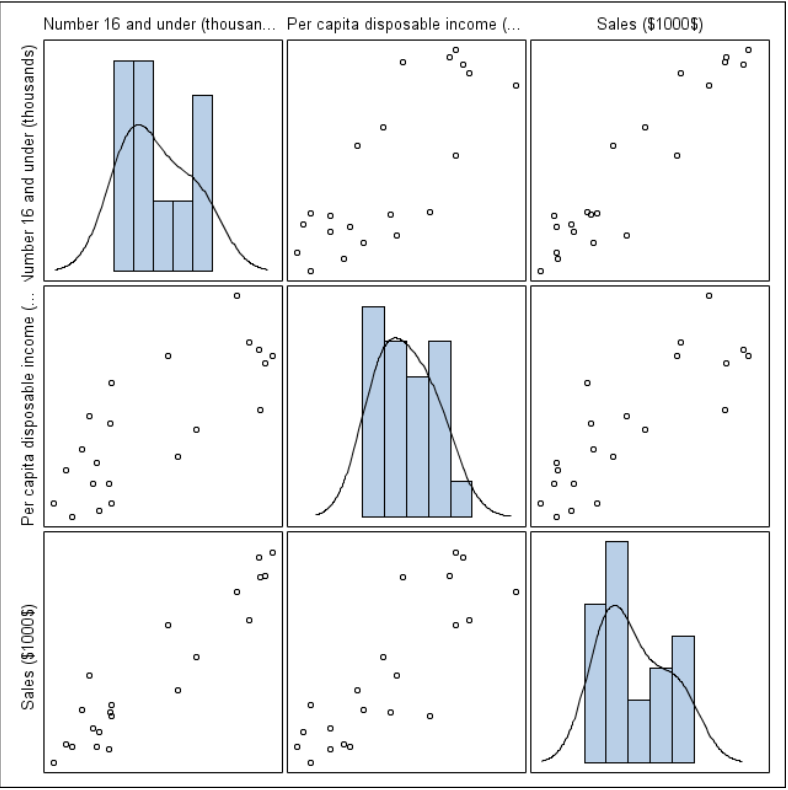
\includegraphics[scale=0.25]{plots/scat-matrix}}
\end{frame}

\begin{frame}{Residuals vs predictors}
\centering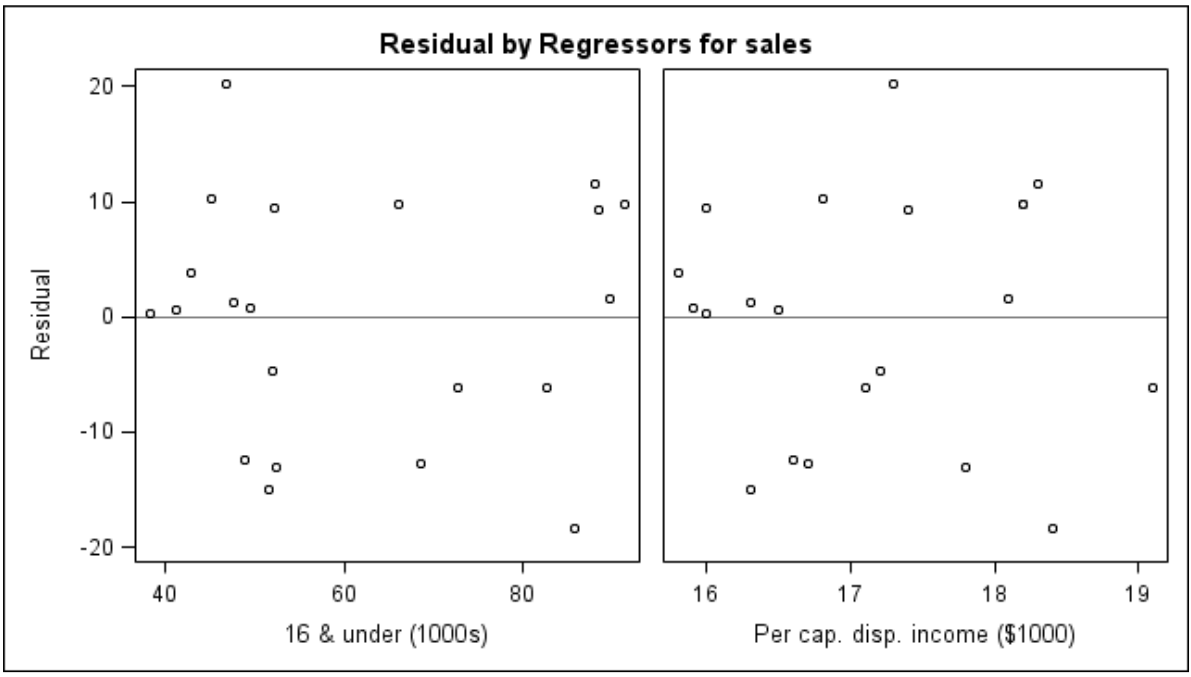
\includegraphics[scale=0.25]{plots/res-x}
\end{frame}

\begin{frame}{Constant variance}
\begin{itemize}
\item Often the most worrisome assumption
\item<2-> Violation indicated by ``megaphone shape'' in residual plot:

\centerline{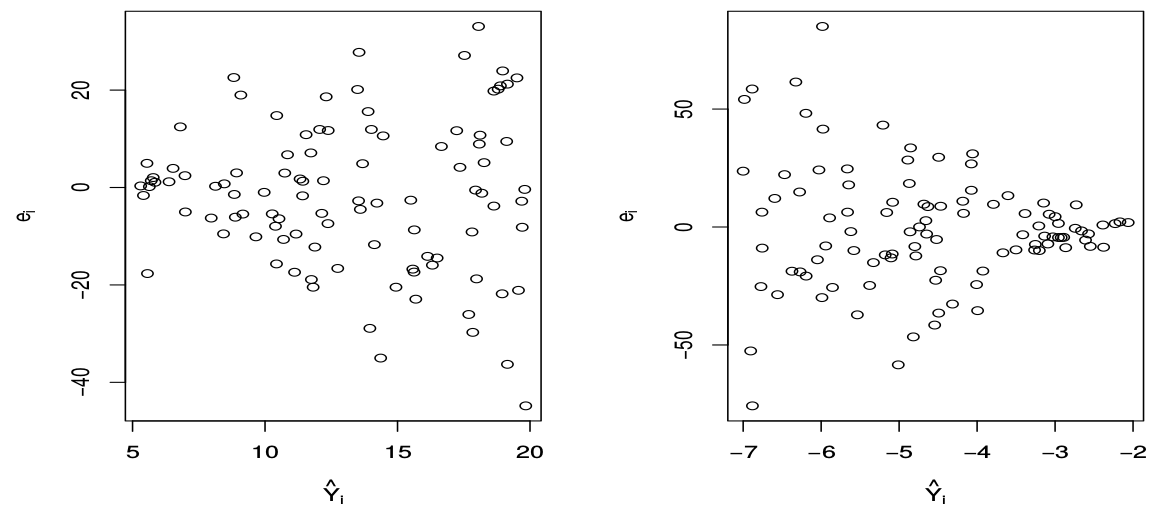
\includegraphics[scale=0.25]{plots/res-fit}}
\item<3-> \structure{Easy remedy:} transform the response, e.g. $Y^\ast=\log(Y)$ or $Y^\ast=\sqrt{Y}$.
\item<4-> \structure{*A more advanced method:} weighted least squares (Chapter 11).
\end{itemize}
\end{frame}

\begin{frame}{Constant variance}
\begin{itemize}
\item \structure{Breusch-Pagan test} (pp.~118--119): tests whether the log error variance increase or decrease linearly with the predictor(s). \pause Let $Y_i\sim\mathcal{N}(\mathbf{x}_i^\top\boldsymbol\beta,\sigma_i^2)$, set 
$$
\ln\sigma_i^2=\alpha_0+\alpha_1 x_{i1}+\ldots+\alpha_k x_{ik}
$$ 
\pause and test 
$$
{\rm H}_0: \alpha_1=\ldots=\alpha_k=0\qquad\Leftrightarrow\qquad\ln\sigma_i^2=\alpha_0,
$$
\pause Requires large samples \& assumes normal errors.
\item\pause \structure{Brown-Forsythe (Levene) test} (pp.~116--117): Robust to non-normal errors. Requires user to break data into groups and test for constancy error variance across groups (not natural for continuous data).
\item\pause Graphical methods have advantage of checking for \textit{general violations}, not just violation of a specific type.
\end{itemize}
\end{frame}

\begin{frame}[fragile]{Breusch Pagan test in {\sc R}}
\begin{footnotesize}
\begin{verbatim}
> library(lmtest)
> dwayne = read.table("path/to/CH06FI05.txt", header=FALSE)
> colnames(dwayne) = c("children", "income", "sales")
> m = lm(sales ~ children + income, data=dwayne)
> bptest(m)

	studentized Breusch-Pagan test

data:  m
BP = 1.949, df = 2, p-value = 0.3774
\end{verbatim}
\end{footnotesize}
\pause With p-value = .3774 we do not reject ${\rm H}_0: \sigma_i=\sigma$ at $\alpha=0.05$, no evidence of non-constant variance.
\end{frame}

\begin{frame}{Normality of errors}
Diagnostics include\ldots
\begin{itemize}
\item Q-Q plot of $e_1,\ldots,e_n$.
\item<2-> Formal test for normality: Shapiro-Wilk (Section 3.5),
essentially based on the correlation coefficient $r$ for expected
versus observed in normal Q-Q plot.
\item<3-> \structure{Remedy:} transformation of $Y$ or any of $x_1, \ldots, x_k$,
*nonparametric methods (e.g. additive models), *robust
regression (least sum of absolute distances), *median
regression.
\end{itemize}
\end{frame}

\begin{frame}{Standard diagnostics}
\centering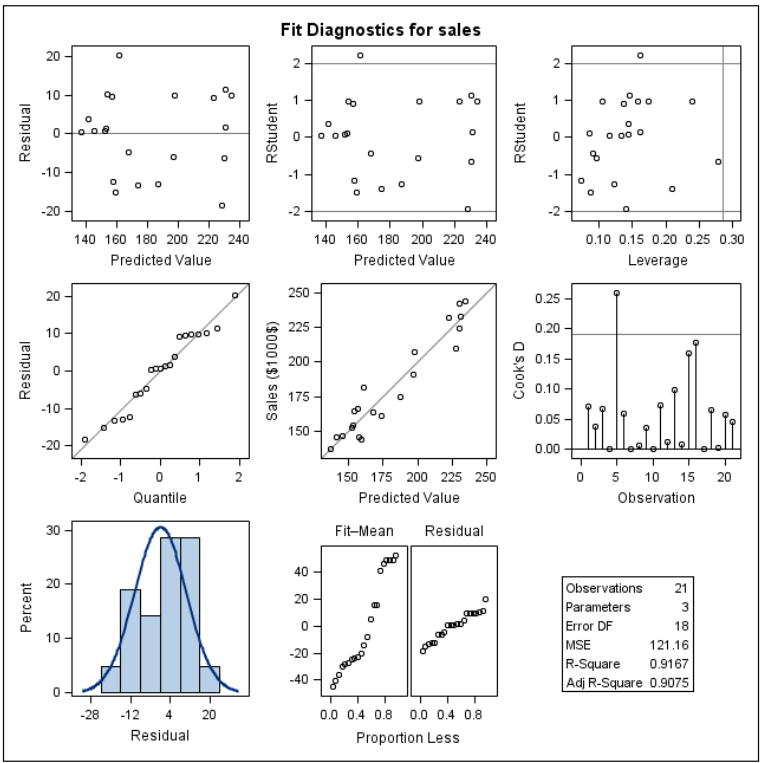
\includegraphics[scale=0.27]{plots/sales-diag}
\end{frame}

\begin{frame}[fragile]
\frametitle{Test for normal residuals in Portrait data}
\begin{small}
\begin{verbatim}
                 Tests for Normality
                 
Test                --Statistic---    -----p Value------
Shapiro-Wilk        W     0.954073    Pr < W      0.4056
Kolmogorov-Smirnov  D     0.147126    Pr > D      >0.1500
Cramer-von Mises    W-Sq  0.066901    Pr > W-Sq   >0.2500
Anderson-Darling    A-Sq  0.432299    Pr > A-Sq   >0.2500
\end{verbatim}
\end{small}
\vspace{10pt}

We do not reject ${\rm H}_0: \epsilon_1,\ldots,\epsilon_n$ are normally distributed
\vspace{10pt}

\pause The Anderson-Darling test looks primarily for evidence of non-normal data in the tails of a distribution; the Shapiro-Wilk emphasizes lack of symmetry in the distribution; i.e. less emphasis placed on the tails.
\end{frame}

\begin{frame}{Comments}
\begin{itemize}
\item With large sample sizes, the normality assumption is not
critical \textit{unless you are predicting new observations}.
\item<2-> The formal test will not tell you the \textit{type} of departure from
normality (e.g. bimodal, skew, heavy or light tails, etc.).
\item<2-> Q-Q plots help answer these questions (if the mean is
specified correctly).
\end{itemize}
\end{frame}

\begin{frame}[fragile]{Independence}
As in the case of SLR, plot of $e_i$ vs $i$:
\begin{figure}
    \centering
    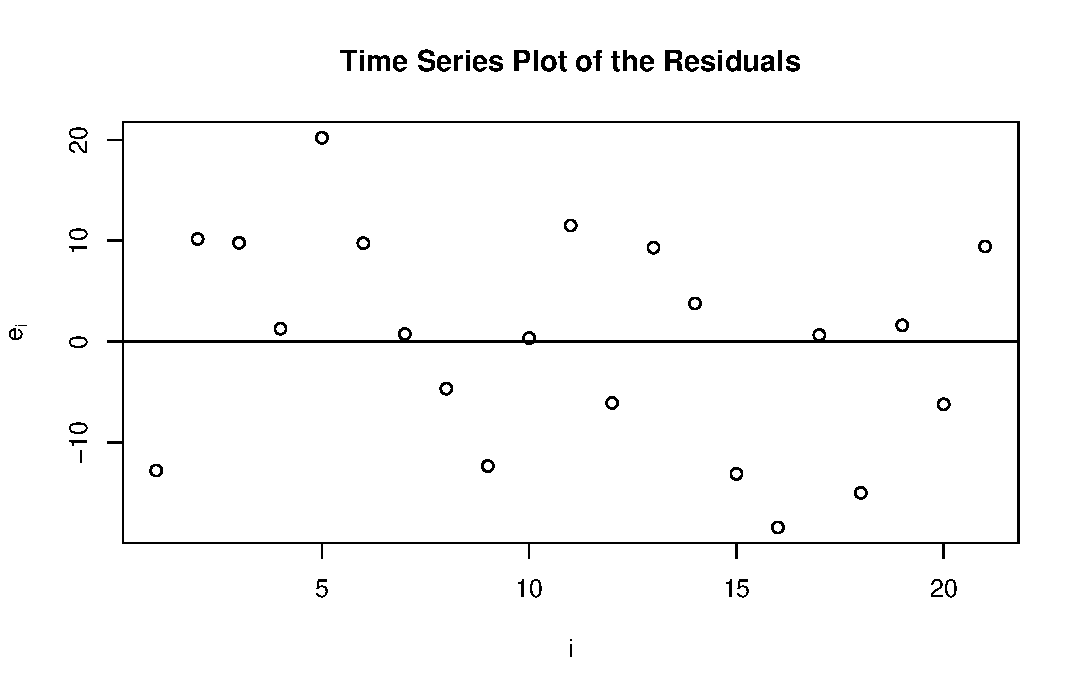
\includegraphics[width=.5\textwidth]{plots/res_ts.pdf}
\end{figure}

\pause and Runs test of independence:
\begin{footnotesize}
\begin{verbatim}
> res = m$residuals
> library(lawstat)
> runs.test(res)

	Runs Test - Two sided

data:  res
Standardized Runs Statistic = -0.66258, p-value = 0.5076
\end{verbatim}
\end{footnotesize}
\end{frame}

\begin{frame}{Transformations of variables}
\begin{itemize}
\item Some violations of our model assumptions may be fixed by
transforming one or more predictors $x_1,\ldots,x_k$ or $Y$.
\item<2-> If the only problem is a nonlinear relationship between $Y$ and
the predictors, i.e. constant variance seems okay, a transformation of one or more of the $x_1, \ldots, x_k$ is preferred.
\item<3-> If non-constant variance appears in one or more plots of $Y$ versus the predictors, a transformation in $Y$ can help\ldots or make it worse!
\item<4-> \textit{Data analysis is an art}. The best way to learn how to analyze
data is to analyze data.
\item<5-> A nonlinear relationship \textit{could} show itself in the scatterplot matrix of $Y_i$ versus $x_{ij}$ for $j = 1, \ldots, k$, or the residuals $e_i$ versus $x_{ij}$.
\item<6-> The chosen transformation should roughly mimic the relationship seen in the plot.
\end{itemize}
\end{frame}

\begin{frame}{Transformations for $x_{i1},\ldots,x_{ik}$}
Examples of transformations for predictors are:
\begin{itemize}
\item $x^\ast=\log(x)$
\item $x^\ast=\sqrt{x}$
\item $x^\ast=1/x$
\item $x^\ast=\exp(x)$ or $x^\ast=\exp(-x)$
\end{itemize}
We will examine \textit{marginal} relationships and transformation ``fixes''. %For multiple regression these might better plots versus predictors, or better yet added variable plots.
\end{frame}

\begin{frame}{Example 1: transforming a predictor}
\centerline{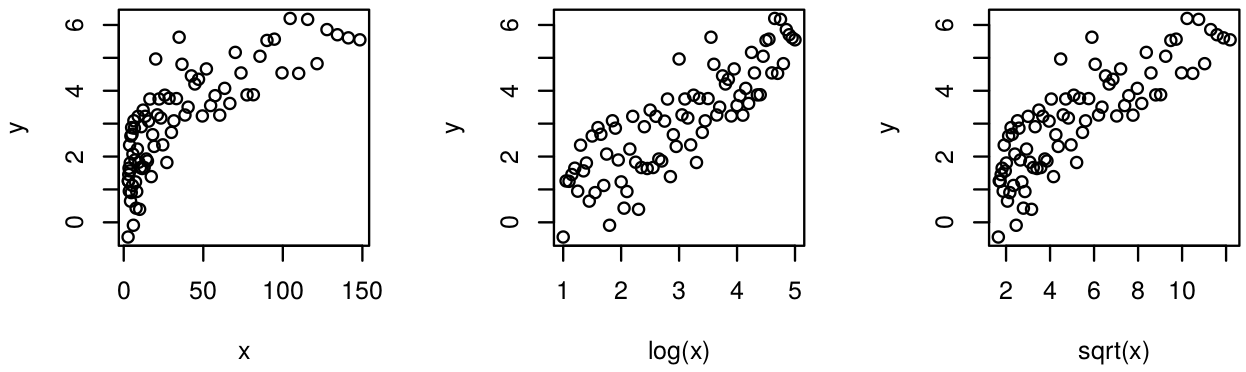
\includegraphics[scale=0.25]{plots/transf1}}
\end{frame}

\begin{frame}{Example 2: transforming a predictor}
\centerline{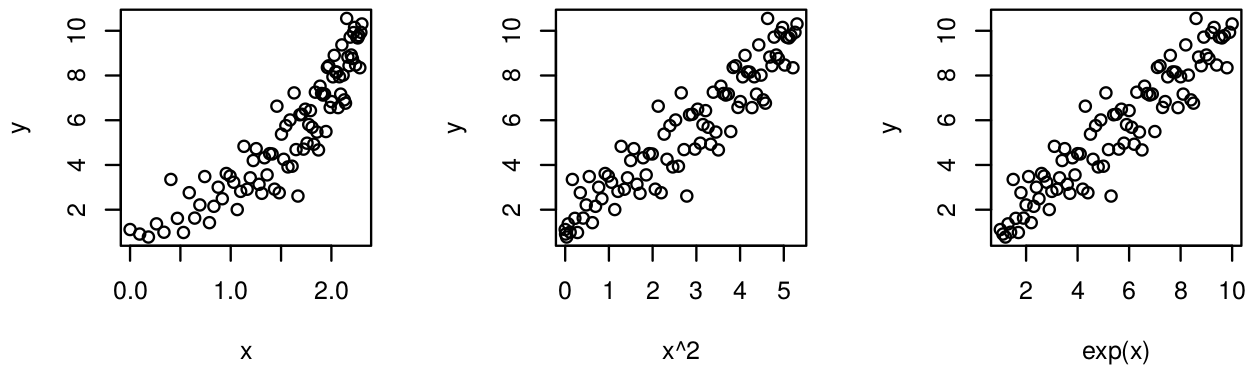
\includegraphics[scale=0.25]{plots/transf2}}
\end{frame}

\begin{frame}{Example 3: transforming a predictor}
\centerline{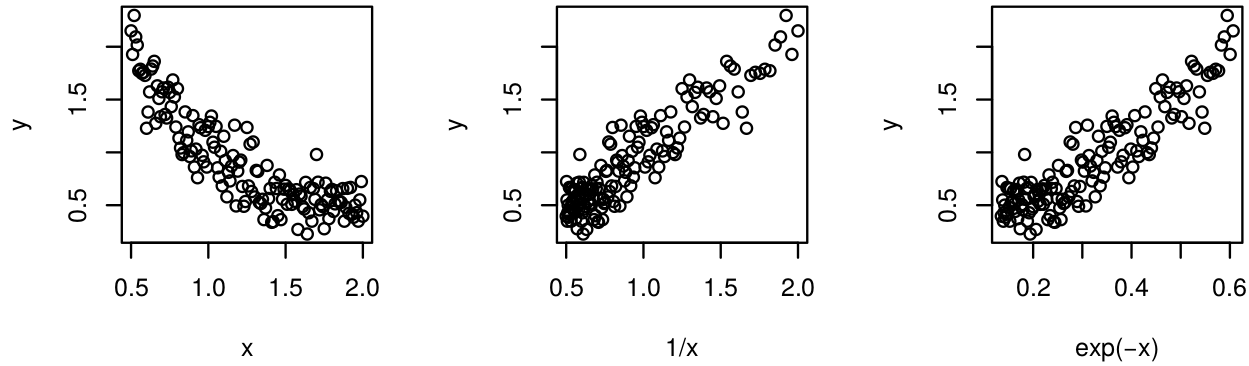
\includegraphics[scale=0.25]{plots/transf3}}
\end{frame}

\begin{frame}{Transforming a response}
If there is evidence of nonconstant error variance, a transformation of $Y$ can often fix things. Examples include:
\begin{itemize}
\item $Y^\ast=\log(Y)$
\item $Y^\ast=\sqrt{Y}$
\item $Y^\ast=1/Y$
\end{itemize}
See Figure 3.15, page 132.
\vspace{10pt}

All of these are included in the Box-Cox family of transformations.
\vspace{10pt}

For some data, a transformation in $Y$ may be followed by one or more transformations in the $x_{i1},\ldots, x_{ik}$.
\end{frame}

\begin{frame}{Example 4: transforming the response}
\centerline{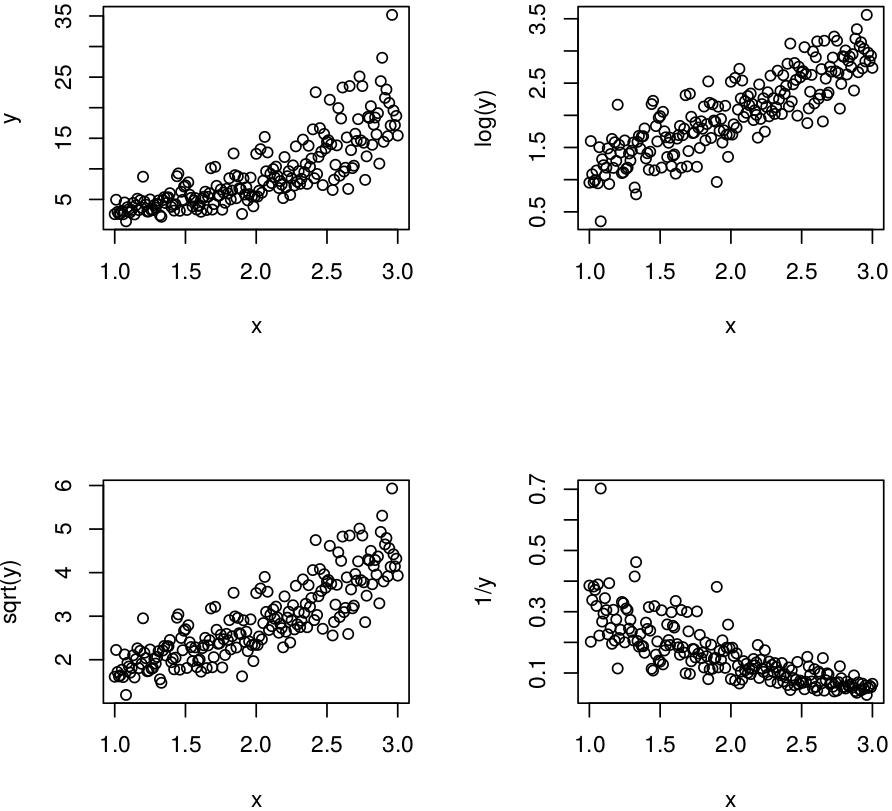
\includegraphics[scale=0.25]{plots/transf4}}
\end{frame}

\begin{frame}{Example 5: transforming the response}
\centerline{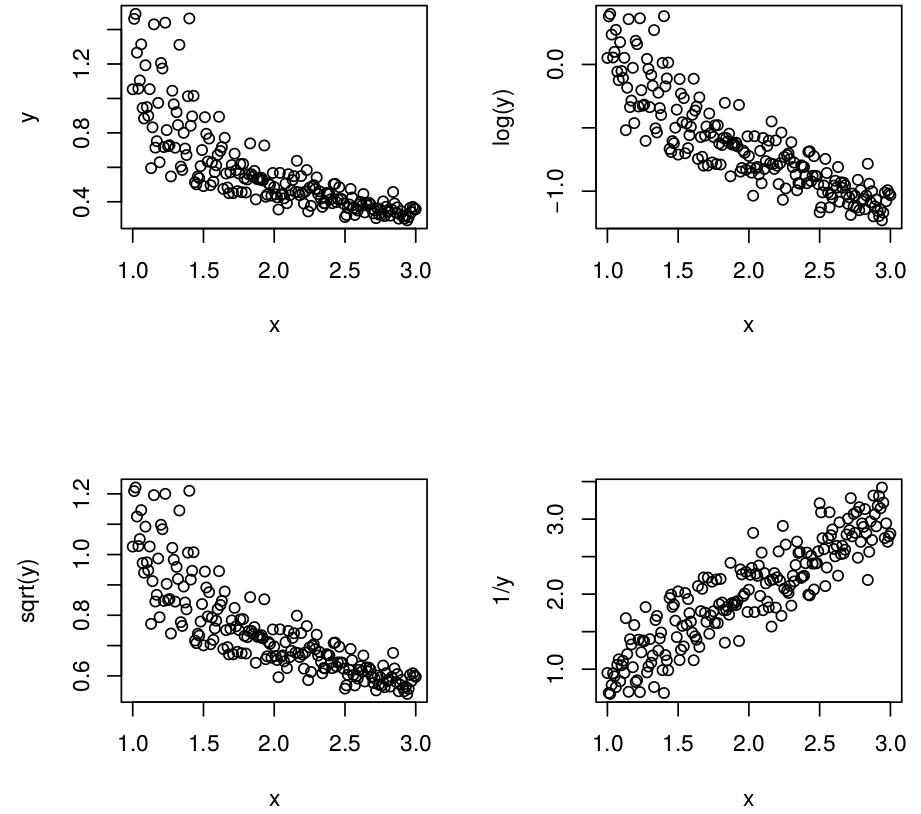
\includegraphics[scale=0.25]{plots/transf5}}
\end{frame}

\begin{frame}{Box-Cox transformations}
\textbf{Box-Cox transformations} are of the type
$$
Y^\ast=\frac{Y^\lambda-1}{\lambda}
$$
where $\lambda$ is estimated from the data, typically $-3\le\lambda\le3$. These include
\begin{align*}
\lambda=2\qquad &Y^\ast=(Y^2-1)/2\sim Y^2\\
\lambda=1\qquad &Y^\ast=Y-1\sim Y\\
\lambda=0\qquad &Y^\ast=\log(Y)\\
\lambda=-1\qquad &Y^\ast=1-1/Y\sim1/Y\\
\lambda=-2\qquad & Y^\ast=1/2-1/(2Y^2)\sim1/Y^2
\end{align*}
{\sc R} will help you to pick $\lambda$ automatically.
\end{frame}
\end{document}